\documentclass[a4paper, adobefonts]{ctexart}

\usepackage[scale=0.75]{geometry}
\usepackage{minted, hyperref, graphicx}

\hypersetup{colorlinks=true, linkcolor=blue}
\newminted{c}{baselinestretch=1.0}

\title{Linux项目作业实验报告}
\author{蔡日骏\quad12348003}

\begin{document}
\maketitle

\section{实验简介}
\label{sec:shi_yan_jian_jie_}
本次实验要求实现\verb|ls|命令的基本功能,能通过\verb|-l|参数切换简要/详细模式。

\section{实现细节}
\label{sec:shi_xian_xi_jie_}

\subsection{遍历目录}
\label{sub:bian_li_mu_lu_}
Linux下常用的遍历目录的方法有以下三种:

\begin{enumerate}
    \item \verb|opendir|/\verb|readdir|/\verb|closedir|函数,使用比较麻烦,除非一边读取
        一边处理数据,否则需要动态分配内存并根据需要动态调整数组大小。
    \item \verb|scandir|函数,使用方便,函数库会自动分配足够的内存,并能根据需要自动进行
        过滤和排序。
    \item \verb|fts_|系列函数,功能强大,能方便地实现递归遍历,但不是POSIX标准函数。
\end{enumerate}

最后我选用的是\verb|scandir|函数,使用libc内置的\verb|alphasort|函数作为比较器进行排序,
并自定义一个过滤器函数用于过滤隐藏文件。调用方式如下:

\begin{ccode}
struct dirent **namelist;
n_items = scandir(path, &namelist, _ignore_hidden, alphasort);
if(n_items == (size_t)(-1)) {
    perror(path);
    return EXIT_FAILURE;
}
\end{ccode}

过滤器\verb|_ignore_hidden|用于过滤隐藏文件,定义如下:

\begin{ccode}
int _ignore_hidden(const struct dirent *item)
{
    return !(item->d_name[0] == '.');
}
\end{ccode}

\verb|scandir|会自动在堆上分配足够的内存,因此数据使用完后需要释放\verb|namelist|数组中
存放的地址以及\verb|namelist|数组本身。

\subsection{分栏对齐}
\label{sub:fen_lan_dui_qi_}
\verb|ls|输出分栏时需要进行对齐。为保持整齐,对齐时计算每列最宽的行的宽度,该列就按照该
宽度进行对齐。

在计算列宽时,一个需要处理的问题是,一个字符的字节长度并不一定等于其输出时的列宽。比如
在UTF-8编码下,一个中文字符的字节长度为3,但等宽字体下一个中文字符占2个英文字母的宽度。

为了解决这个问题,需要使用\verb|mbrtowc|函数从多字节字符串中提取一个宽字符,然后使用
\verb|iswprint|和\verb|wcwidth|函数计算该宽字符的输出宽度。为方便起见,定义了下面这个函数:

\begin{ccode}
size_t mbs_pwidth(const char *s, size_t n)
{
    mbstate_t mbs;
    wchar_t wc;
    size_t clen, width = 0;
    const char * const s_end = s + n;

    memset(&mbs, 0, sizeof(mbs));
    while((clen = mbrtowc(&wc, s, s_end - s, &mbs))) {
        switch(clen) {
            case (size_t)(-1):  /* truncated string (incomplete character) */
                s = s_end;
                ++width;
                break;
            case (size_t)(-2):  /* invalid character */
                ++s;
                ++width;
                break;
            default:  /* valid wide character */
                s += clen;
                if(iswprint(wc))
                    width += wcwidth(wc);
        }
    }

    return width;
}
\end{ccode}

为了使C的宽字符库正常工作,程序启动时需要使用\verb|setlocale(LC_ALL, "");|进行本地化设置。

此外,在摘要模式中进行分栏输出时,为了计算需要分的栏数,还需要获取用户当前终端窗口的宽度。
这个宽度可以通过\verb|ioctl|系统调用进行获取。在获取失败时,使用默认宽度80。定义下面这个函数:

\begin{ccode}
int cal_max_width()
{
    struct winsize ws;
    if(!ioctl(STDOUT_FILENO, TIOCGWINSZ, &ws) && ws.ws_col > 0)
        return ws.ws_col;
    return 80;  /* fallback (fail to get the width of tty) */
}
\end{ccode}

\subsection{详细信息}
\label{sub:xiang_xi_xin_xi_}
在详细模式下(提供\verb|-i|参数),使用\verb|lstat|系统调用查询文件的详细信息,
并使用\verb|getpwuid|和\verb|getgrgid|函数获取UID和GID对应的用户名和组名。

\section{演示}
\label{sec:yan_shi_}

下面为程序运行效果。测试平台分别为Mac OS X Yosemite (Darwin 14.0.0, clang 6.0)和
Arch Linux (Linux Kernel 3.17.6, gcc 4.9.2)。

\begin{figure}[htp!]
    \centering
    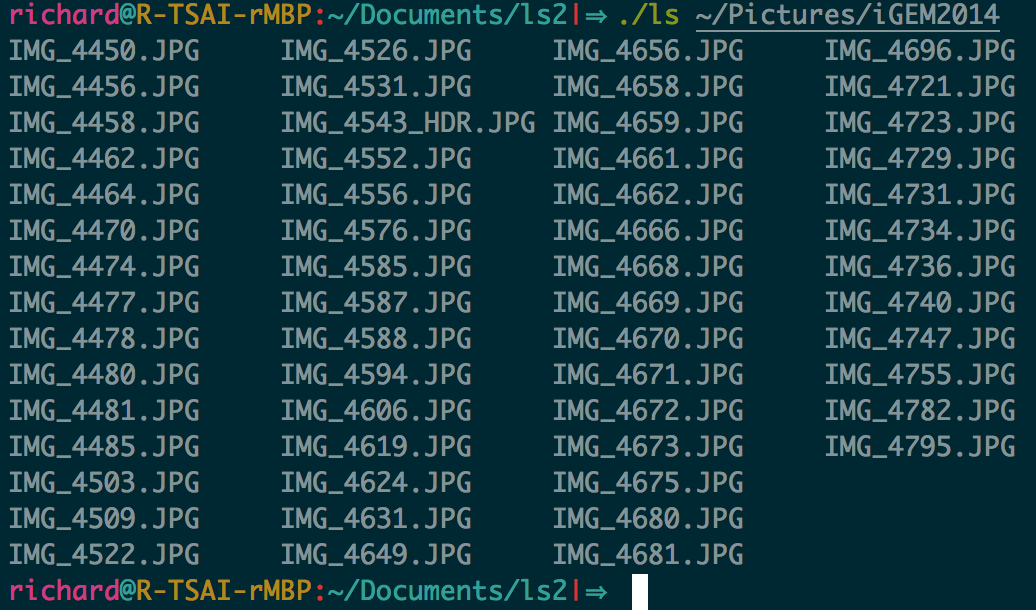
\includegraphics[scale=0.6]{1.png}
    \caption{Mac OS X Yosemite 1}
    \label{fig:1}
\end{figure}

\begin{figure}[htp!]
    \centering
    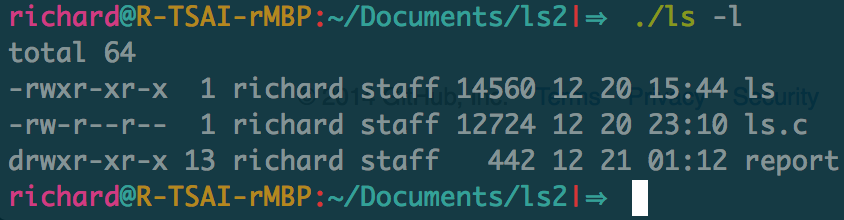
\includegraphics[scale=0.6]{2.png}
    \caption{Mac OS X Yosemite 2}
    \label{fig:2}
\end{figure}

\begin{figure}[htp!]
    \centering
    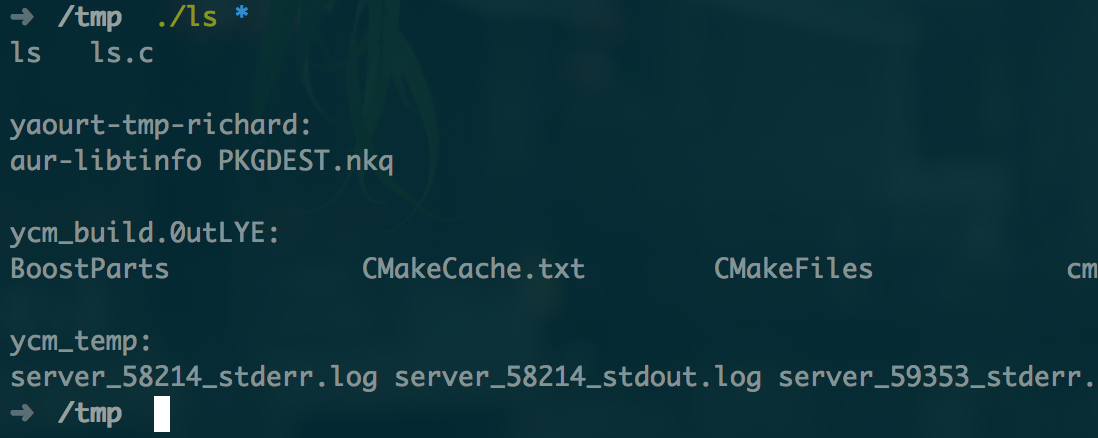
\includegraphics[scale=0.6]{3.png}
    \caption{Arch Linux 1}
    \label{fig:3}
\end{figure}

\begin{figure}[htp!]
    \centering
    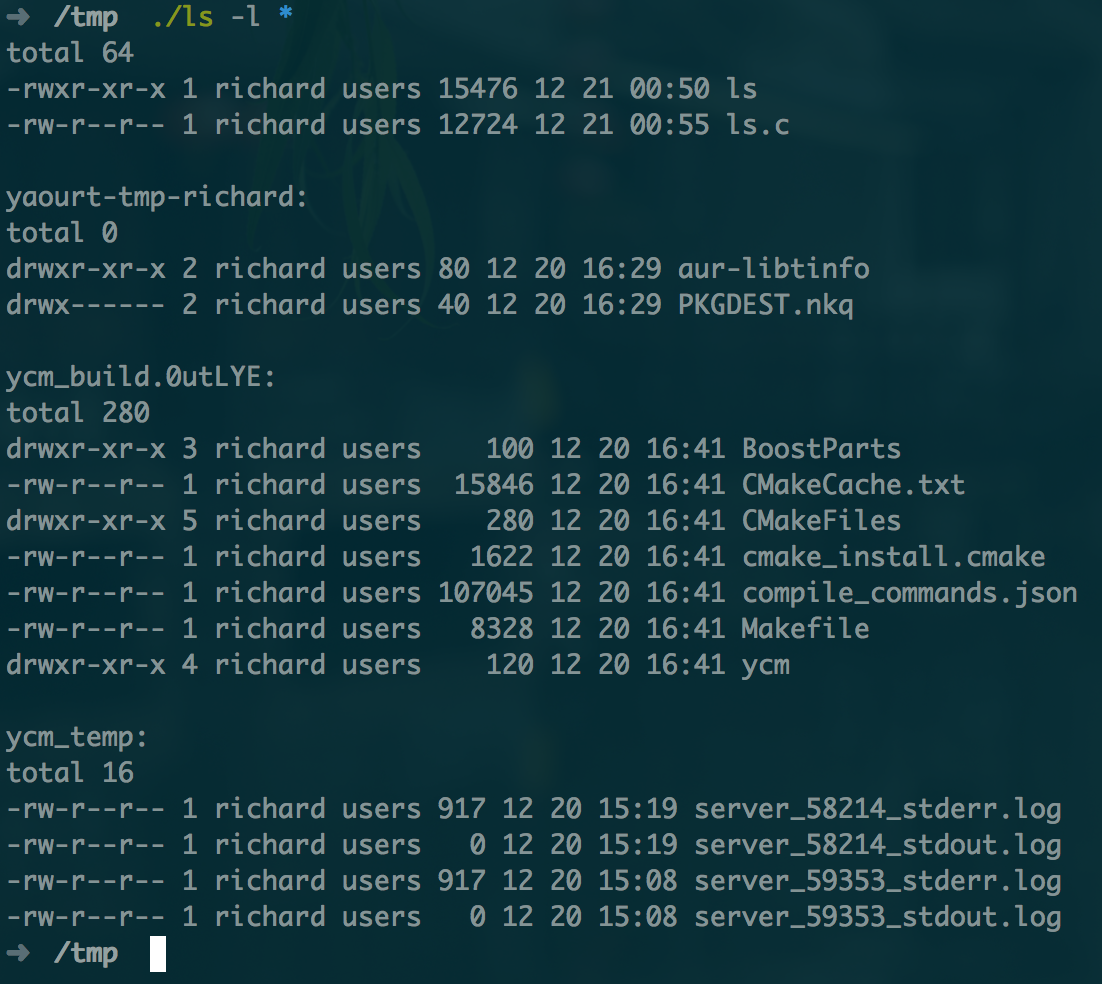
\includegraphics[scale=0.6]{4.png}
    \caption{Arch Linux 2}
    \label{fig:4}
\end{figure}

\end{document}
